\chapter{CMB}

\section{Introduction}

In 1949 the existence of CMB was predicted by George Gamow, Ralph Alpher, and Robert Herman.

The light emitted during the recombination phase of the universe appears today "stratched" into the microwave part of the electromagnetic spectrum.

When photons and baryons were coupled, the first ones where not able to travel. 

In 1964 Arno Penzias and Robert Wilson discovered the CMB by accident using a horn antenna. They kept picking up a persistent, low-level noise coming from every direction in the sky. 

After cleaning out the antenna from interference, they realized they had found the relic radiation predicted decades earlier.

In 1989 the \textbf{COBE} satellite was launched to measure the CMB with high precision. It was the first to detect that this radiation was not perfectly smooth.

In 1998, \textbf{BOOMERang}: high-altitude balloon launched from
Antarctica (dry and high). With its higher resolution it was the first experiment to clearly detect the "first acoustic peak" in the CMB power spectrum. It was also the first to discover that CBM's fluctuations had a certain "scale".

2001, \textbf{WMAP} satellite: improved sensitivity and angular resolution. First full-sky detection of E-mode polarization

2009, \textbf{Planck} satellite: most detailed image of the CMB sky today measuring intensity and polarization (E and B-mode) of the radiation

\subsection{CMB monopole}

CMB shows an almost perfect black body spectrum radiation at $T = 2.725$ K.

% todo: add plot

In a scale of \textasciitilde 3.35mK, we can observe some fluctuations in the CMB temperature. This is a Doppler effect due to our peculiar motion through space, which is made up of:

\begin{itemize}
    \item Motion of Earth around the Sun ($\sim$30 km/s)
    \item Motion of the Sun around the Milky Way center ($\sim$220 km/s)
    \item Motion of the Milky Way towards the Virgo cluster ($\sim$300 km/s)
\end{itemize}

The total vector sum of these motions gives a net velocity of $\sim$369 km/s.

\subsubsection{anisotropies}

At a smaller scale of \textasciitilde 10$\mu$K we can further observe some tiny quantum fluctuations, that, scaled by inflation, become density perturbations of the universe.

Prior to recombination (i.e. formation of neutral hydrogen), the baryon-photon fluid undergoes acoustic oscillations driven by gravity and radiation pressure.

The temperature pattern we observe today provides a picture of the density perturbation at recombination ($z \simeq 1100$).

%todo: add plots

To statistically analyze the CMB anisotropies:

\begin{itemize}
    \item Measure the anisotropies distribution over the sky
    $$
        \frac{\Delta T}{T}(\theta, \phi) = \frac{T(\theta, \phi) - \bar{T}}{\bar{T}}
    $$
    
    \item Expand in spherical harmonics
    $$
        \frac{\Delta T}{T}(\theta, \phi) = \sum_{\ell=0}^{\infty} \sum_{m=-\ell}^{\ell} a_{\ell m} Y_{\ell m}(\theta, \phi)
    $$

    the higher is $a_{\ell m}$ the more $Y_{\ell m}$ contributes.
    
    \item Compute the angular power spectrum
    $$
        C_\ell = \frac{1}{2\ell + 1} \sum_{m=-\ell}^{\ell} \langle |a_{\ell m}|^2 \rangle
    $$
\end{itemize}

lower $\ell$ meand large angular scales, going to the right we can observe smaller scales.

%todo: add angular scale plot

---

The Temperature-Temperature power spectrum is sample-variance limited (we have only a universe to observe):

we can measure these fluctuations by averaging multiple "sphere" samples from the CMB. The larger the spheres (larger scale), the lower the number of samples and the larger the uncertainty.

\begin{itemize}
    \item At low multipoles (i.e. large angular scales) only few modes can be measured, and the sample variance increases.
    \item For almost every scale Planck's sensors were so sensitive that the only remaining source of error is Cosmic Variance itself.
\end{itemize}

The uncertainty due to sample variance dominates, thus it whould be useless to develop more precise satellites to study the CMB.

\subsubsection{Polarization}

Consider incoming radiation from the left being scattered by 90 degrees out of the screen from a free electron

The free electron is accelerated in the direction of the photon’s electric field. This makes the electron emit a new photon linearly polarized

If the incoming radiation from the left and top are of equal intensity, the result is no polarization in the outgoing direction

In case of isotropic radiation we do not expect a net polarization of the scattered light

Only if the intensity of the radiation varies at 90 degrees, i.e. the distribution has a \textbf{quadrupole pattern}, does a net linear polarization result

In particular there is a net linear polarization (\textasciitilde10\%) that is aligned with the cold axis of the quadrupole anisotropy

The relevant epoch for the generation of polarization in the CMB is around recombination since at early times scattering is too efficient to allow a significant quadrupole to grow, while after recombination scatterings are very rare (until the universe reionizes).

There are two main physical mechanisms for producing a quadrupole anisotropy: density fluctuations and gravitational waves.

the linear polarization vary across the sky in a pattern which is the projection of the quadrupole anisotropies at recombination

%todo: add plane wave modulation

Polarization is a spin-2 field. We can split it in two orthogonal bases:

\begin{itemize}
    \item \textbf{E mode}: Polarisation direction parallel or
    perpendicular to the wavevector; even parity (gradient-like).
    \item \textbf{B mode}: Polarisation direction 45° tilted with respect to the wavevector; odd parity (curl-like).
\end{itemize}

The density wave creates E mode polarization, while gravitational waves create B mode polarization. Thus, we can decouple the different patterns and study the different phenomena.

%todo: add grav wave stretching plot

We can measure three different power spectra in polarization:

\begin{itemize}
    \item \textbf{EE}: Power spectrum of the E-E autocorrelation mode polarization. It is noide limited (sample-variance limit at $\ell \approx 3000$)
    \item \textbf{TE}: ...
    \item \textbf{BB}: ... noise limited, undetected.
\end{itemize}

Due to noise, all the polarization spectra are weaker than the TT signal.

$\langle EB \rangle$ and $\langle TB \rangle$ vanish for parity-preserving fluctuations.

\subsection{Measuring the CMB}

\subsubsection{mapping CMB temperature}

In temperature, the foreground dominates almost all frequencies. There is only a "sweet spot" between 70 and 100 Ghz, where CMB dominates over foregrounds.

It is also possible to measure the thermal dust (and/or synchrotron) emissions at higher (lower) frequencies and then clean up the signal from the noise.

In polarization, it is not true the same.

\subsubsection{mapping CMB polarization}

CMB polarization can be mapped in terms of \textbf{Stokes parameters} $Q$ and $U$, which are local measurements of the orientation of the electric field at a specific point in the sky:

\begin{itemize}
    \item \textbf{Q}: Measures polarization along the 0° -- 90° axes
    \item \textbf{U}: Measures polarization along the 45° -- 135° axes
\end{itemize}

The Stokes $Q$ and $U$ parameters are related to the E and B modes through:

\begin{align}
    Q(\hat{\theta}) &= \int \frac{d^2\ell}{(2\pi)^2} (E_\ell \cos 2\phi_\ell - B_\ell \sin 2\phi_\ell) \exp(i\boldsymbol{\ell} \cdot \hat{\theta}) \\
    U(\hat{\theta}) &= \int \frac{d^2\ell}{(2\pi)^2} (E_\ell \sin 2\phi_\ell + B_\ell \cos 2\phi_\ell) \exp(i\boldsymbol{\ell} \cdot \hat{\theta})
\end{align}

The polarized amplitude $P = \sqrt{Q^2 + U^2}$ measures the total polarization intensity.

\subsubsection{B-modes in detail}

B-modes allow us to study the early ages of the universe, before recombination (electromagnetic field cannot "see" before recombination).

%todo: add b-mode plot (slide 22)

some B-mode are due to lensing effects on E-mode polarizations.

Search for B-modes:

\begin{itemize}
    \item There are only upper limits from searchers for B-modes in the CMB Polarization

    \item Assuming simple inflationary gravitational wave models the Tensor-to-Scalar ratio parameter, r, is the only parameter which controls the amplitude of the BB spectrum at large scale
    \item 2$\sigma$ upper limit from BICEP1 (2014): $r < 0.7$
\end{itemize}

\textbf{BICEP2} is an instrument built specifically to study B-mode polatizations. It targets the "southern Hole", a region thought to be free of foreground contamination.

At 150 GhHz the foregroung contamination was predicted to be at minimum in the Southern Hole.

%todo: add BICEP2 results

The level contamination in the Southern Hole was not as low as they expected.

%todo: add BICEP2 + plank results

The instruments used to study the CMB are:

CMB-S4: South Pole telescope
LiteBIRD: Satellite

We do not need high resolution, since we are interested in large angular scales.

\section{Epoch of Reionization}

After the last scattering epoch, in the Dark Ages, the universe is basically \textbf{neutral} and there where no photons emitted by astrophysical sources due to too low energy.

At the end od the Dark Ages, the first starts start to be created . They are observable todat at a (very high) redshift $z \approx 25-30$.

Duting the Reionization phase we have the creation of the most of the stars, and in the Post-Reionization phase we have the creation of galaxies.

%todo: add reionization plot and enhance paragraph below

Knowing the distributiojn field of the Dark Ages can be useful: the most recent universe is strongly affected by astrophysics (baryon effects).

Evidence of reionization of IGM are:

\begin{itemize}
    \item CMB photons scatter off free electrons in the IGM.
    \item The measured quantity in CMB observations is the optical depth due to Thomson scattering off free electrons:
    $$
        \tau = \int_0^{z_{re}} n_e(z) \sigma_T \frac{c \, dz}{(1+z) H(z)}
    $$
    where $H$ is the Hubble parameter and $\sigma_T$ is the Thomson scattering cross section.

    We can actually decouple the integral:
    $$
    \tau = \int_0^{z_{lss}} dz = \int_0^{z_{re}} dz + \cancelto{0}{\int_{z_{re}}^{z_{CMB}} dz}
    $$
    \item Because this scattering is a random process along the line of sight, it effectively damps the primary fluctuations of the CMB at all scales. The $C_\ell^{TT}$ power spectrum is suppressed by a factor:
    
    $$
        C_\ell^{TT,\text{obs}} = e^{-2\tau} C_\ell^{TT,\text{primordial}}
    $$
\end{itemize}

The dumping effect is degenerate (behaves similarly) with the amplitude of the density fluctuations (generated in the inflation epoch), parametrized with $A_s$ or $sigma_8$:

$$
C_{\ell}^{TT, obs} \propto A_s e^{-2 \tau}
$$

TE spectrum can break the degeneracy: on large scale ($\ell < 10$) reionization create a “bump” since the scattering of CMB photons after reionization polarize the light at these scales for the first time since the Big Bang

%todo: add plot

By assuming a model for the reionization history, $n_e(z)$, it is possible to estimate the reionization redshift $z_{re}$.

Current analyses often assume an "instantaneous reionization" model, where $n_e = n_H$ for $z < z_{re}$, and $n_e = 0$ for $z > z_{re}$, and the transition is relatively quick ($\Delta z_{re} = 0.5$) and symmetrical (tanh function):

$$
x_e(z) = \frac{1 + f_{He}}{2} \left[ 1 + \tanh\left( \frac{(1 + z_{re})^{3/2} - (1 + z)^{3/2}}{\Delta w} \right) \right]
$$

Current constraints from Planck give $z_{re} \approx 7.7$.

\subsubsection{Lyman-$\alpha$ Forest}

The Lyman-$\alpha$ forest is a series of absorption lines observed in the spectra of distant quasars (QSOs), caused by neutral hydrogen in the intergalactic medium along the line of sight.

\textbf{Ly-alpha absorption lines:}

\begin{itemize}
    \item \textbf{Example:} For a QSO at $z_Q = 3$ emitting a photon at wavelength $\lambda_Q = 1187$ \AA $< \lambda_{H}$, the light reaches the Ly$\alpha$ wavelength $\lambda_H = 1216$ \AA\ at redshift:
    $$
        z \approx 1187 \times \frac{4}{1216} - 1 \approx 2.9
    $$
    If neutral hydrogen is present at that position in space, it will produce a distinct absorption signature in the spectrum.
    
    \item We observe this specific feature in the QSO spectrum at $\lambda = \lambda_Q(1 + z_Q) \approx 4742$ \AA. Therefore, any absorption arising at a specific redshift $z$ will appear in our observations at:
    $$
        \lambda = \lambda_H (1 + z)
    $$
\end{itemize}

\begin{figure}[H]
    \centering
    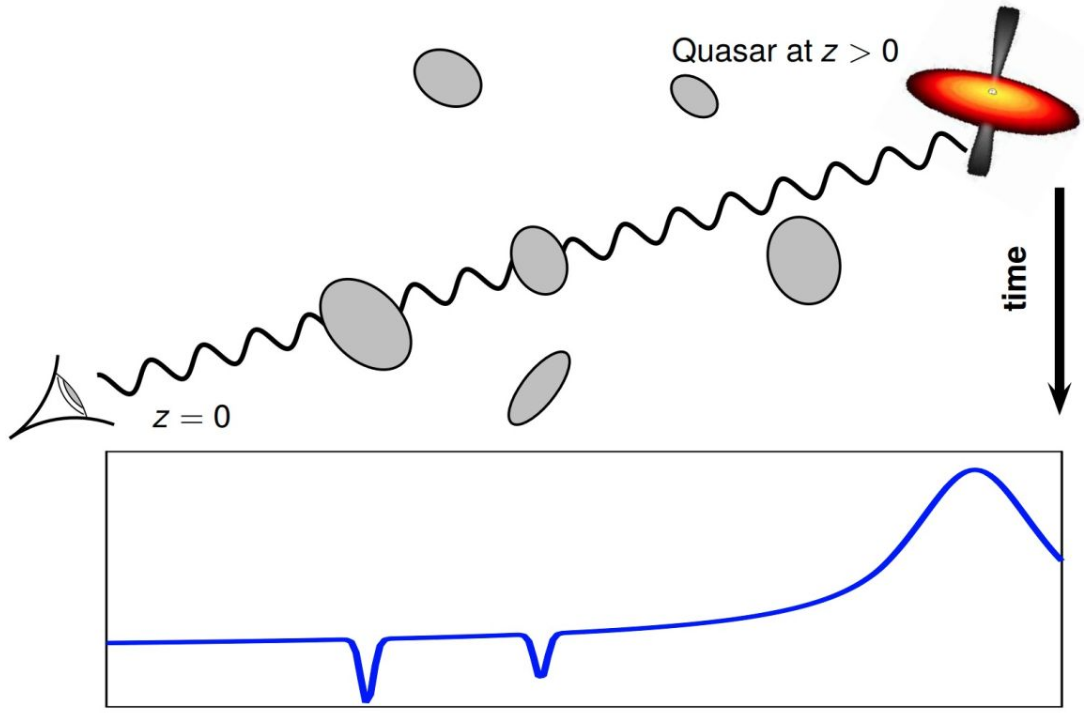
\includegraphics[width=0.45\textwidth]{assets/lyman.png}
    \hfill
    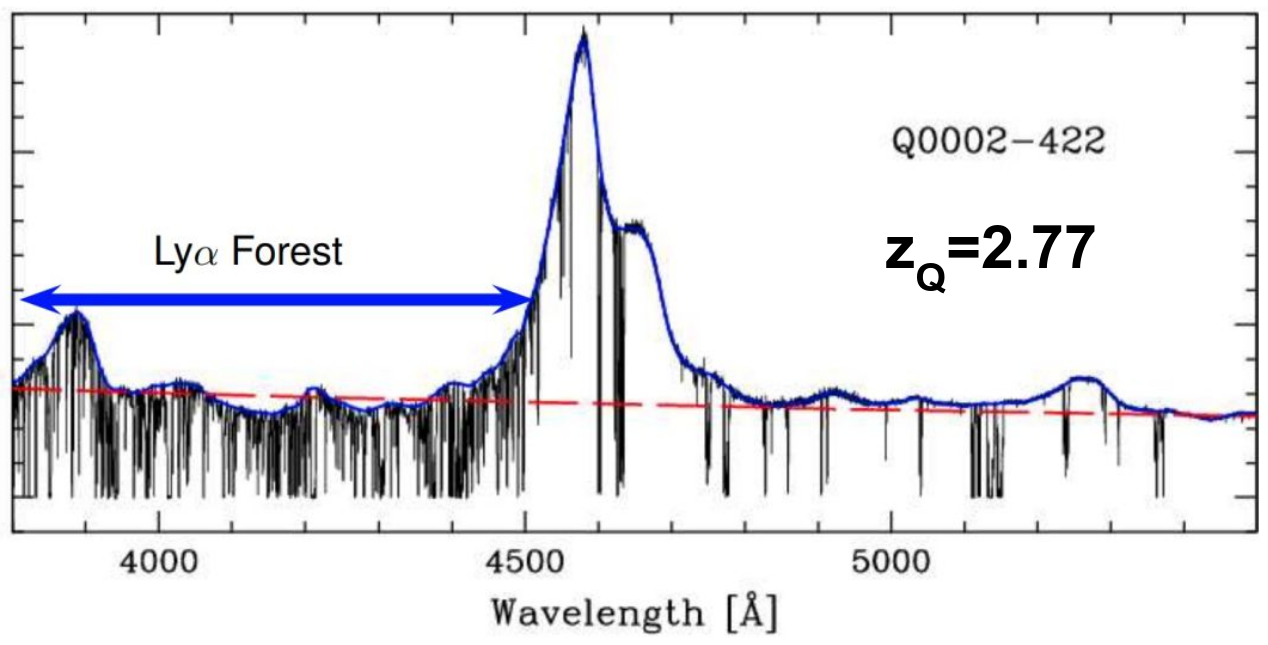
\includegraphics[width=0.5\textwidth]{assets/lyman-2.png}
\end{figure}

The absorption lines blueward of the emission line arise from Ly \& transition of HI present between the QSO and us

The unabsorbed parts of the spectrum correspond to either ionized regions or no matter at all

\subsubsection{Gunn-Peterson effect}

If the IGM is filled with neutral hydrogen, every single wavelength "blue-ward" of the Ly-$\alpha$ line is eventually absorbed, leading to a zero flux in the spectrum.

We can determine the reionization epoch by looking at the spectra of QSOs at different redshifts

A non-zero flux is observed till $z \sim 5.5$

The cross-section for Ly-a scatterin high that even a tiny fraction of neutral hydrogen (X, = p,, / py = 10*) is enough to create a complete Gunn-Peterson trough.

$$
F \propto r^{-\tau_{GP}}
\qquad
\tau_{GP} \approx \left( \dfrac{\bar X_{HI}}{10^{-5}} \right)
$$

The Ly-a transition saturates easily, and cannot be used to assess the exact level of reionization, but just a lower limit ($X_{HI} > 10^{-4}$)

\subsubsection{Perspectives}

\textbf{Interpretation of current data:}

\begin{itemize}
    \item QSO absorption spectra imply $X_{HI} > 10^{-4}$ at $z \sim 6$
    \item CMB data imply $z_{re} \sim 8$ assuming an instantaneous reionization (too simplistic!)
    \item There is no tension between the two results; the data collectively suggest that reionization is an extended process, starting at $z > 8$ and completing around $z \sim 6$
\end{itemize}

\textbf{Open questions:}

\begin{itemize}
    \item \textbf{Epoch of reionization:} When did the sources produce enough photons to ionize the Universe? ($6 < z < 20$)
    \item \textbf{Nature of reionization:} Was the process sudden or gradual? Homogeneous or inhomogeneous?
    \item \textbf{Sources of reionization:} The primary drivers are still debated — first stars, quasars, exotic particles?
\end{itemize}